\chapter{Design}

\section{Gameplay Overview}
\todo[inline]{Maybe draw an example as this is a bit confusing}
The game provides a fairly straightforward experience from the user's point of view.
Conceptually, it is a card game, so I will describe it as such.
The game consists of three decks which I dub `in play', `out of play' and `reserve'. In addition to this, there are $n$ `pillars' - these are attributes of importance within the game story's context. Each of these has a minimum, maximum and current value.
The `in play' deck has a defined starting set of cards, with the `reserve deck' containing all others - `out of play' starts empty.
Both decks are shuffled at the start of the game, and each pillar has a predefined starting value.

The player draws and reads a card from the play deck, each one showing the following information:

\begin{itemize}
    \item Title
    \item Description
    \item Choice \#1 (`accept')
    \item Choice \#2 (`reject')
    \item Requirements to draw
\end{itemize}
Each choice on a card consists of text detailing the response, and the effects of the response. Effects are made up of two parts - pillar changes, and cards added/removed. Pillar changes specify amounts to add or remove from one or more pillars. Cards added/removed defines which cards should be moved between `out of play' and `reserve'.
Requirements to draw consists of conditions that the current pillar levels must satisfy in order for this card to be drawn.

After each choice made (turn), any cards in `out of play' the meet the current pillar requirements are moved to `in play', and any `in play' that do not are moved to `out of play'. 

The game ends when any of the pillars fall to their minimum value.

\section{UI}

\subsection{Game}
As described above, the game sounds like a lot of effort on behalf of the player, having to sort and shuffle cards. Fortunately, this effort can be removed completely through work done by the computer. This leaves a simple game from the user perspective; users are presented with a card, make a choice, and get the next card.

This meant that the design for the game UI would also be simple. Figure \ref{fig:game_drawing} shows my first design for this UI. Initially, I wasn't sure whether the pillars should be visible to the user, however after some testing it was clear that they were needed to provide the player with feedback throughout the game, so they were later added to the top of the screen.

\begin{figure}[!h]
	\centering
	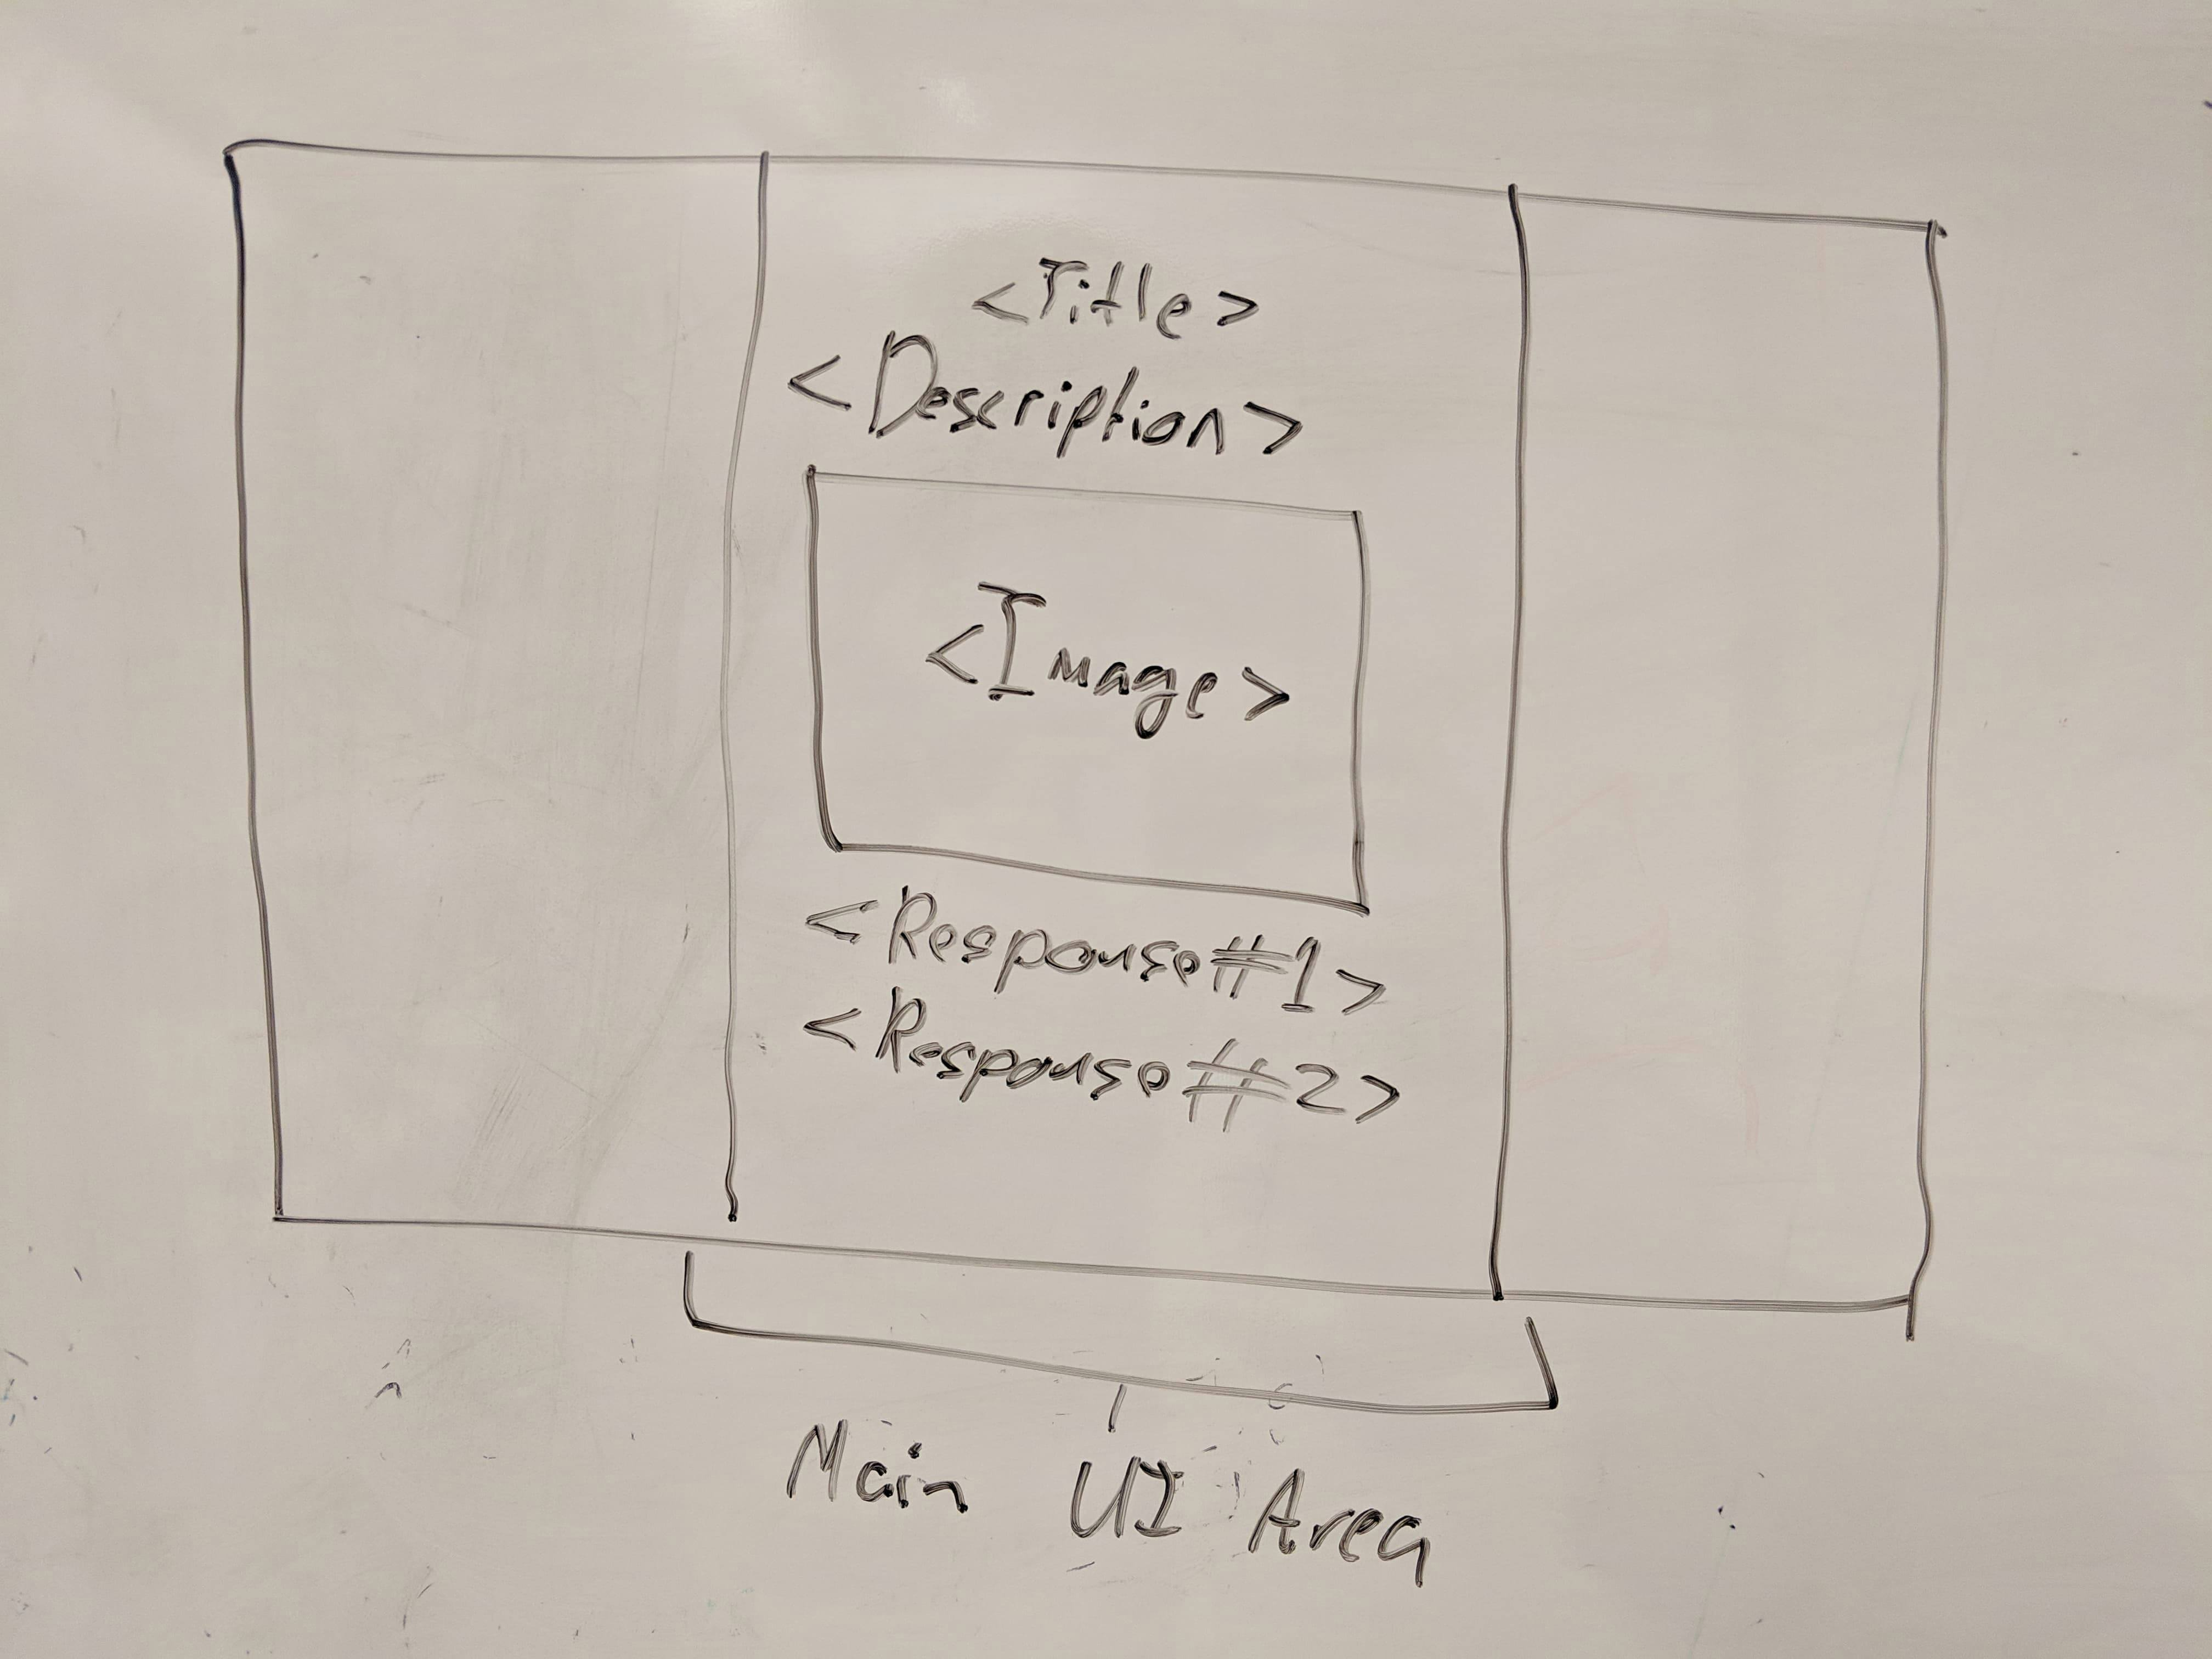
\includegraphics[width=1.0\textwidth]{./images/design/game_drawing.jpg}
	\caption{Initial design for game screen}
	\label{fig:game_drawing}
\end{figure}

\subsection{Admin tools}

\subsubsection{Game Maker}
The game maker interface was the most difficult to design, as I wanted the user to be able to maintain a high-level overview of the game while adding and editing pillars and cards. 
After thinking this through, I initially settled on the design depicted in figure \ref{fig:game_maker_drawing}. The idea here is that editing is done in the left panel, while the right side continues to show an interactive view of the game, including a visualisation of the relationships between cards.
The final design ended up being roughly the same, however the card view is not as complex - connections between cards are not visualised, as after more consideration of the relationships involved, I could think of no clear way of showing this.
Instead in the final design the cards are merely displayed in a grid.

\begin{figure}[!h]
	\centering
	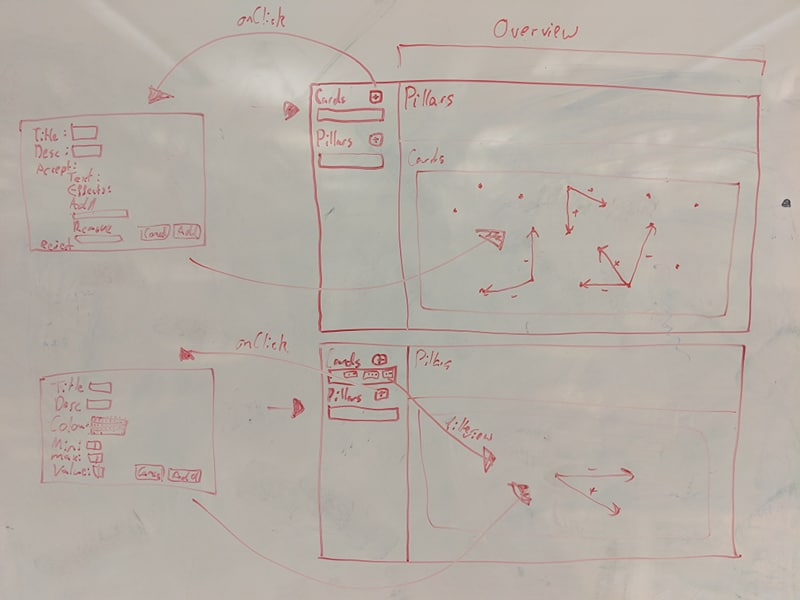
\includegraphics[width=1.0\textwidth]{./images/design/game_maker_drawing.png}
	\caption{Initial design for game maker}
	\label{fig:game_maker_drawing}
\end{figure}

\subsubsection{Visualisation}

The visualisation screen took a similar shape to the game maker, with data selection and filtering happening in a left panel while the visualisations are updated on the right.
It is possible to filter results to be visualised by pillar values. This limits the data shown only to cards that appeared while pillar values match the specified criteria The visualisations I chose to show are as follows:
\begin{itemize}
    \item Accept/Reject balance

    This is a horizontal bar chart showing the proportion of players that choose one option over the other for a given set of cards. Each card has a value between -1 and 1, where -1 indicates that players choose the reject option every time, while 1 indicates accept is chosen every time.

    \item Total times drawn
    
    This is a vertical bar chart showing the total number of times each card has been drawn and responded to.
    
    \item Pillar average

    This shows the average pillar levels over all turns.
\end{itemize}

The intention of these visualisations is to allow a user to `play' with the data. The live updating charts allow the user to rapidly identify relationships, for example between pillar levels and accept/reject balance.

\section{Frontend}
When using Redux, one of the first design decisions that must be made is the structure of the Redux store. This is the JavaScript object that holds the page's state. Figures \ref{fig:store_shape} and \ref{fig:card_example} show a visual representation of the store for the game site. The game logic runs client-side, so to enable this, the entire game definition is requested from the database server once the player requests to play it. Depending on the use case, this could be considered a downside as technically a player could `cheat' the game through using console commands. This choice did however greatly simplify the API between the client and sever, as once the game has begun, the client only needs to send the outcome of each turn.

\begin{figure}[!h]
	\centering
	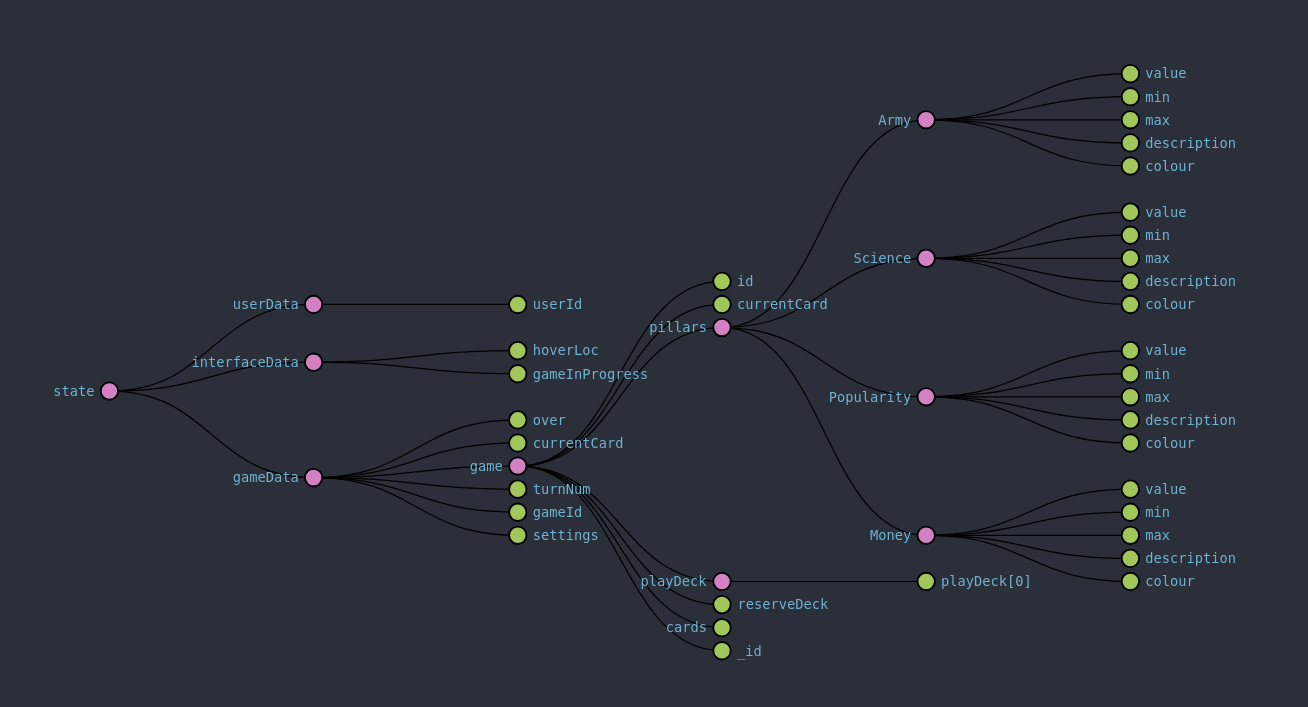
\includegraphics[width=1.0\textwidth]{./images/design/store_shape.png}
	\caption{Redux store object structure. Note that the pillars (Army, Science, Popularity, Money) are game definition dependent. Cards object is omitted due to large size.}
	\label{fig:store_shape}
\end{figure}

\begin{figure}[!h]
	\centering
	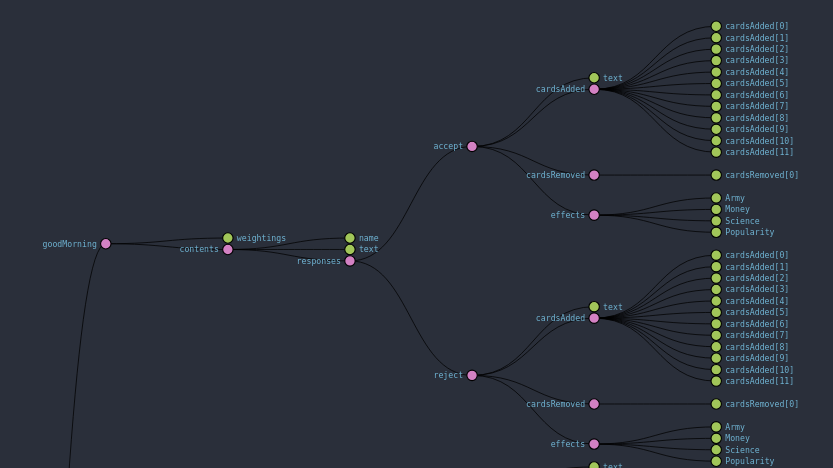
\includegraphics[width=1.0\textwidth]{./images/design/card_example.png}
	\caption{Example of a card object in the store. This is a starting card that adds many other cards to the game no matter which option is chosen.}
	\label{fig:card_example}
\end{figure}



\section{Backend}